\makeatletter
\newcommand*{\textoverline}[1]{$\overline{\hbox{#1}}\m@th$}
\makeatother

\section{Hardware module}\label{sec:overview}
\begin{figure}[h]

\includegraphics[width=0.5\textwidth]{system_overview.PNG}
\caption{The Power-Mixing-DAC is build out of 15 branches all connected to the resistor.}
\label{fig:system_overview}
\end{figure}
When looking inside Fig.\ref{fig:traditional}b, the architecture of the Power-Mixing-DAC becomes clear (see Fig. \ref{fig:system_overview}). It is composed out of several functional blocks: a digital front end structure, a level shifter and an amplifier. 
The digital front end synchronizes the data and modulates it with a local oscillator, which operates as square wave at 2GHz. To synchronise the data, D flip-flops will be used. The D flip-flop has two outputs: Q and \textoverline{Q}. A NAND gate mixes Q and LO for the PMOS end stage and a NOR gate mixes \textoverline{Q} and LO for the NMOS end stage. Before the mixed signals reach the final amplification stage, a level shifter translates the signals from a 1.2V $V_{DD}$ which are used for the thin-oxide transistors in the digital front end to a 5V $V_{DD}$ which is used in the final amplification stage. This amplifications stage provides the output power to the 50 $\Omega$ matched antenna.
The Power-Mixing-DAC translates a 15 bit unary coded digital signal with a maximum bandwidth of 500MHz to an analogue signal. Unary coded  signals can provide higher linearity compared to binary coded signals. One of the reasons is that in the creation process of the transistors, it is more precise to make two transistors of the same size, than to make one with exactly two times the size. Due to the maximum resolution of 16 bits the signal to noise ratio (SNR) is limited to a theoretical maximum of 25.8 dB, see Eq.~\ref{eq:SNR}.
\begin{equation}\label{eq:SNR}{SNR = 6.02 \times n + 1.76 = 25.8 dB}\end{equation}
The specified output current is 50 mA, which means that the output power on the 50 $\Omega$ matched antenna should be 20.97 dBm. The aim is to get an IMD3 of at least 30 dBc.

%\begin{figure*}[t]
 %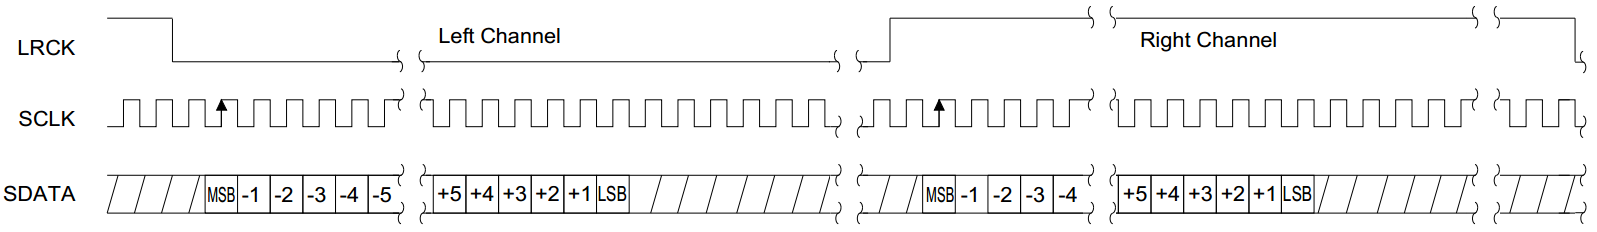
\includegraphics[width=\textwidth]{clocks}
 %\caption{A representation of the LRCK, SCLK and SDIN signals. It shows the required phase synchronization the signals and sampling moments of SDIN.}
 %\label{fig:clocks}
%\end{figure*}